\documentclass{beamer}

\usepackage{amsmath}
\usepackage{amssymb}
\usepackage{amstext}
\usepackage{amsthm}
\usepackage{palatino}
\usepackage{subfigure}
\usepackage{graphicx}
\usepackage{hyperref}
\hypersetup{colorlinks=false}
\usepackage{url}
\usepackage[utf8]{inputenc} 

\newcommand{\Z}{\mathbb{Z}}
\newcommand{\R}{\mathbb{R}}
\newcommand{\N}{\mathbb{N}}
\newcommand{\lam}[2]{\lambda#1.#2}
\newcommand{\BETA}{\boldsymbol\beta}
\newcommand{\barrow}{\rightarrow_\beta}
\newcommand{\Barrow}{\barrow^*}
\newcommand{\I}{\textsf{\textbf{I}}}
\newcommand{\W}{\textsf{\textbf{W}}}

% Bruges til Python-kode.
\newcommand{\pycode}[1]{\textbf{\texttt{#1}}}


\begin{document}
\title{Visualization of $\beta$-reduction Graphs in the Lambda Calculus}   
\author{Niels Bjørn Bugge Grathwohl og Jens Duelund Pallesen} 
\date{\today} 

\frame{\titlepage}

\frame{\frametitle{Table of contents}\tableofcontents} 


\section{Introduktion}
\frame{\frametitle{Introduktion} 
\begin{itemize}
	\item Der findes visulaiseringer af lambda kalkyler, men ingen visualiseringer af reduktionsgrafer
	\item Produktet er udviklet med hensyn til forskere og undervisere inden for området
\end{itemize}
}


\section{Design}
\frame{\frametitle{Design} 
\begin{itemize}
	\item Opdelt design, gør det muligt at udskifte individuelle dele uaflhængigt af hinanden
	\item Et design, som er let at udvide med f.eks. nye tegnealgoritmer
	\item Multiplatform (Python og GTK)
\end{itemize} 
}

\subsection{Grafgenerator}
\frame{\frametitle{Grafgenerator} 
\begin{itemize}
	\item Parser $\rightarrow$ Finde redexer $\rightarrow$ Reducer
	\item Generering af tilfældige grafer
\end{itemize} 
}

\subsection{Graftegner}
\frame{\frametitle{Graftegner} 
\begin{itemize}
	\item GraphViz - Tilbyder en række tegnealgoritmer
	\item Majoriazation - Vores egenimplementerede tegnealgoritme, som tilbyder ekstra fleksibilitet i forhold til GraphViz' tegnealgoritmer
	\item PyGTK - Brugt til GUI pga. god understøttelse samt at det er enkelt at benytte
	\item Python Widgets - Brugt til at binde de forskellige GUI elementer sammen
\end{itemize} 
}

\subsection{GUI}
\frame{\frametitle{GUI} 
\begin{itemize}
	\item Det er ikke en GUI opgave - Fokus har været på 
	\item Enkel GUI
\end{itemize} 
}

\section{Eksempler}
\frame{\frametitle{Eksempler} 
\begin{itemize}
	\item Predecessor og Successor
	\item Addition, multiplikation og potens
	\item Hypercube
	\item Assosiation
	\item Cons
\end{itemize} 
}

\subsection{Predecessor og Successor}
\frame{\frametitle{Predecessor og Successor} 
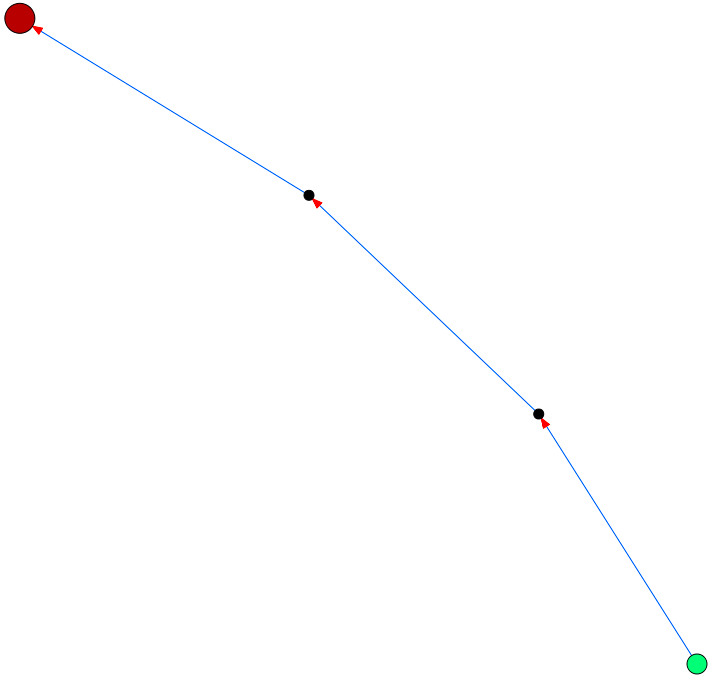
\includegraphics[height=2in]{Succ5_NEATO.png}
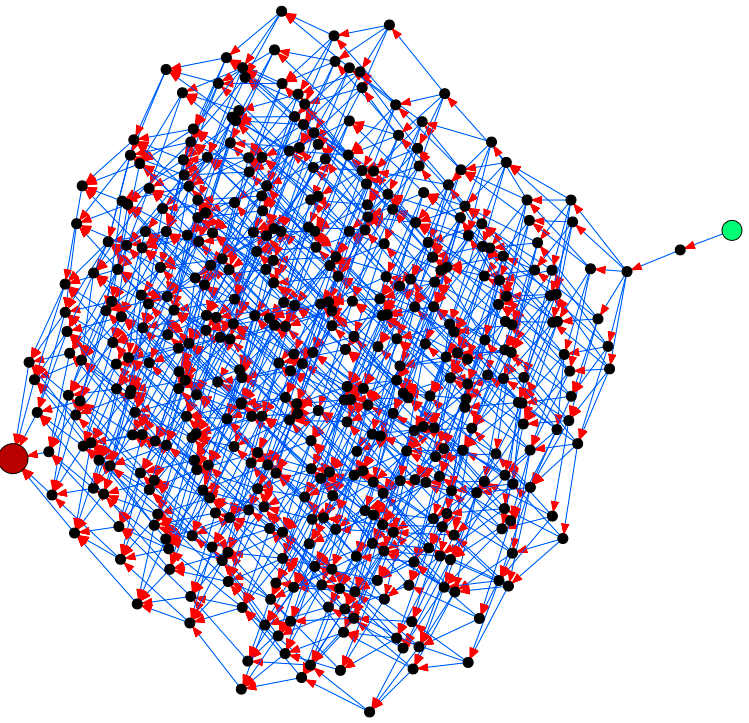
\includegraphics[height=2in]{Pred5_NEATO.png}
}

\subsection{Addition, multiplikation og potens}
\frame{\frametitle{Addition, multiplikation og potens}
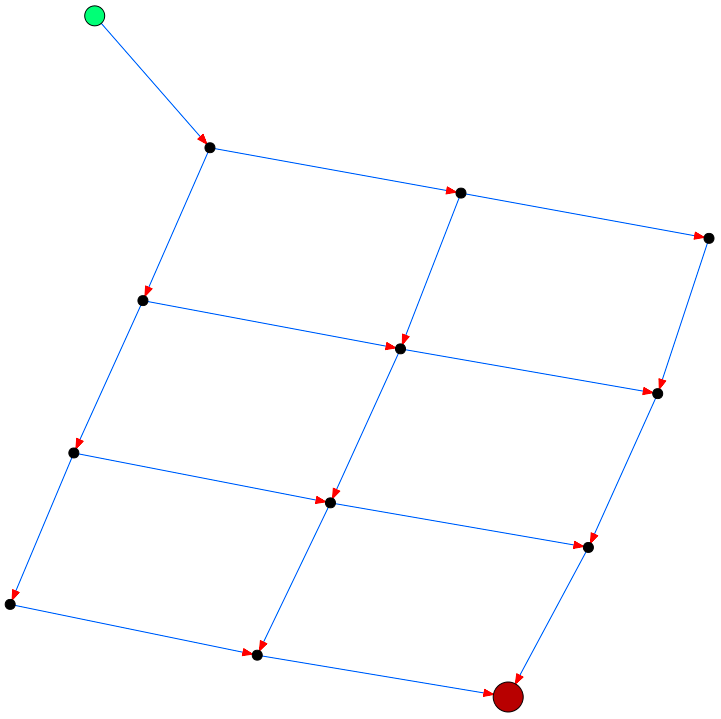
\includegraphics[height=1.5in]{Sum22_NEATO.png}
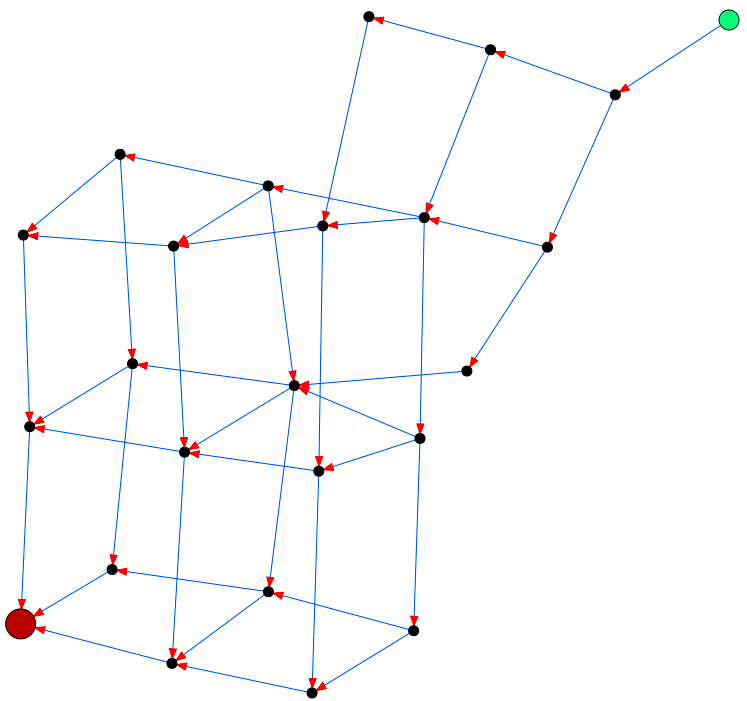
\includegraphics[height=1.5in]{Prod22_NEATO.png}
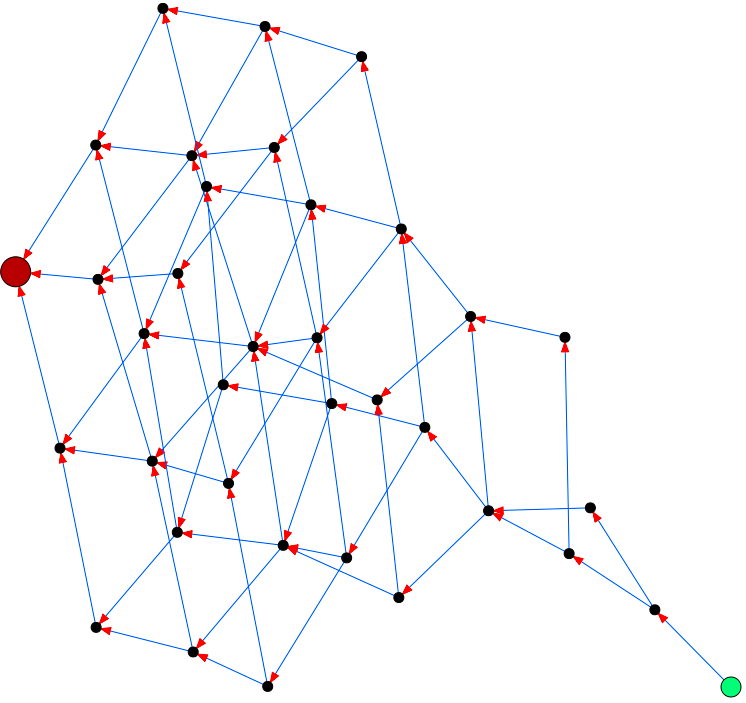
\includegraphics[height=1.5in]{Exp22_NEATO.png}
}

\subsection{Hypercube}
\frame{\frametitle{Hypercube ($((\lam{x_1}{x_1}) f)\hdots((\lam{x_n}{x_n}) f)$)}
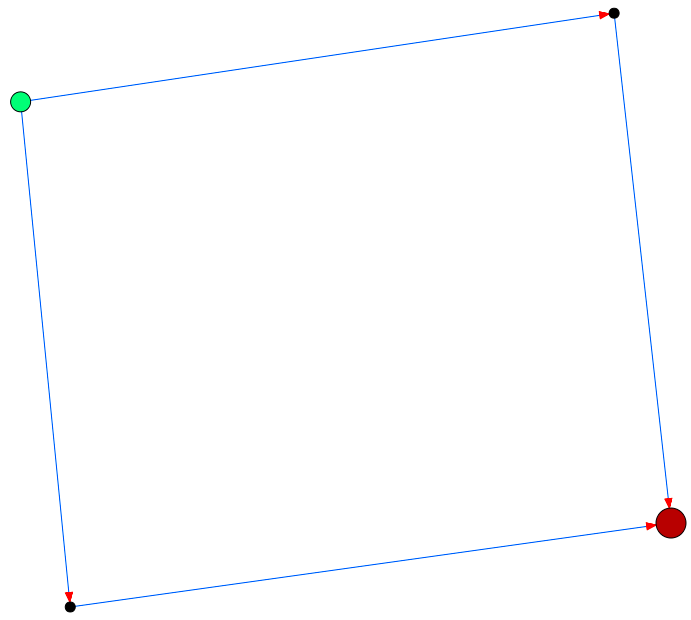
\includegraphics[height=1.5in]{Cube2d_NEATO.png}
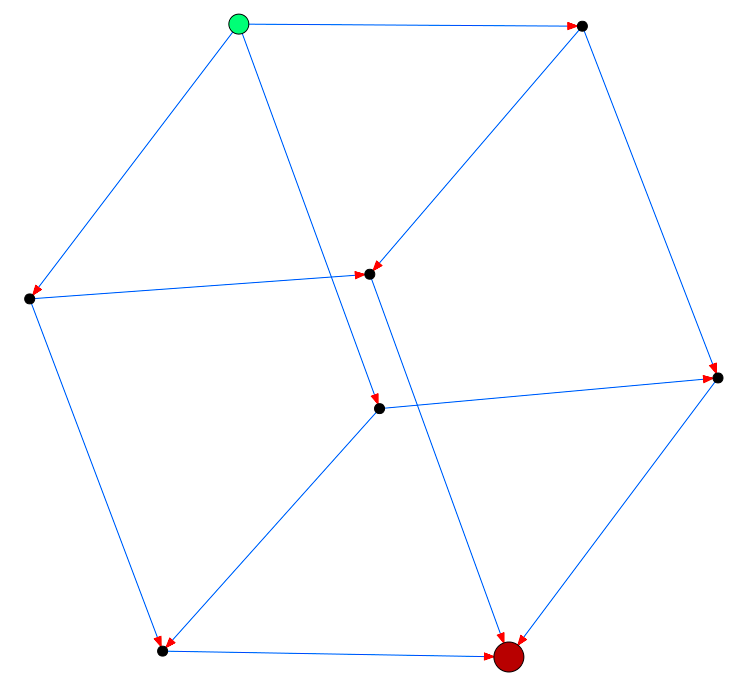
\includegraphics[height=1.5in]{Cube3d_NEATO.png}
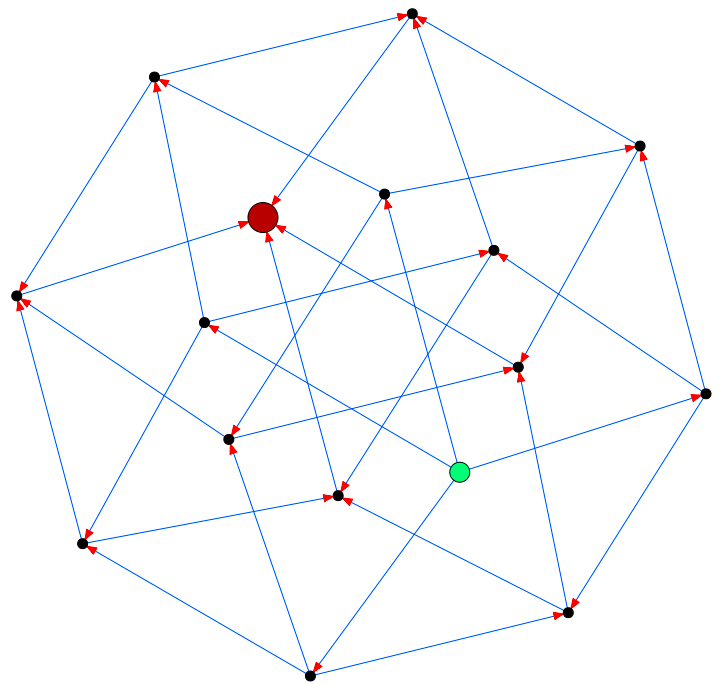
\includegraphics[height=1.5in]{Cube4d_NEATO.png}
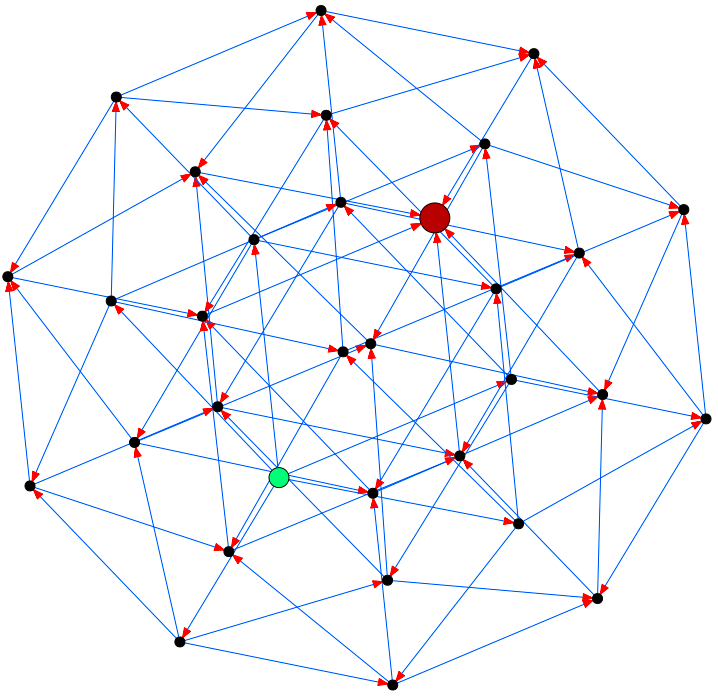
\includegraphics[height=1.5in]{Cube5d_NEATO.png}
}

\subsection{Assosiation}
\frame{\frametitle{Assosiation}
\begin{figure}[htbp!]
	\subfigure[$\omega_3 \omega_3 \omega_3 \omega_3$]{
		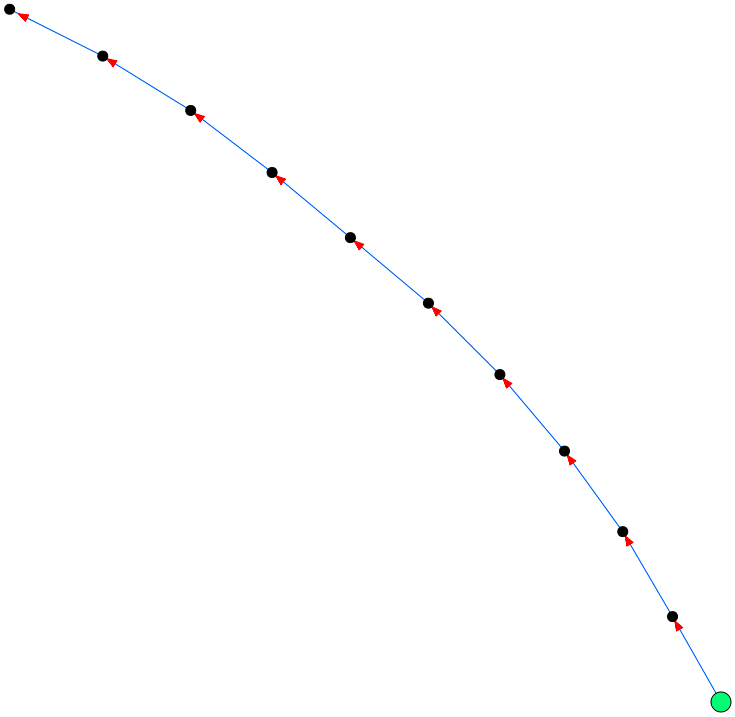
\includegraphics[height=1.2in]{Snake_2_NEATO.png}
	}
	\subfigure[$\omega_3 \omega_3 (\omega_3 \omega_3)$]{
		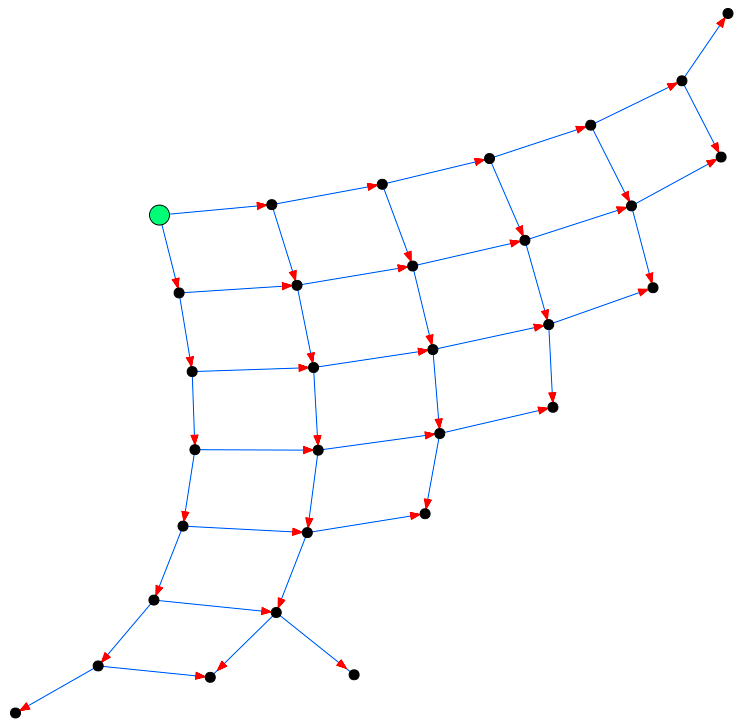
\includegraphics[height=1.2in]{Snake_3_NEATO.png}
	}
	\subfigure[$\omega_3 (\omega_3 (\omega_3 \omega_3))$]{
		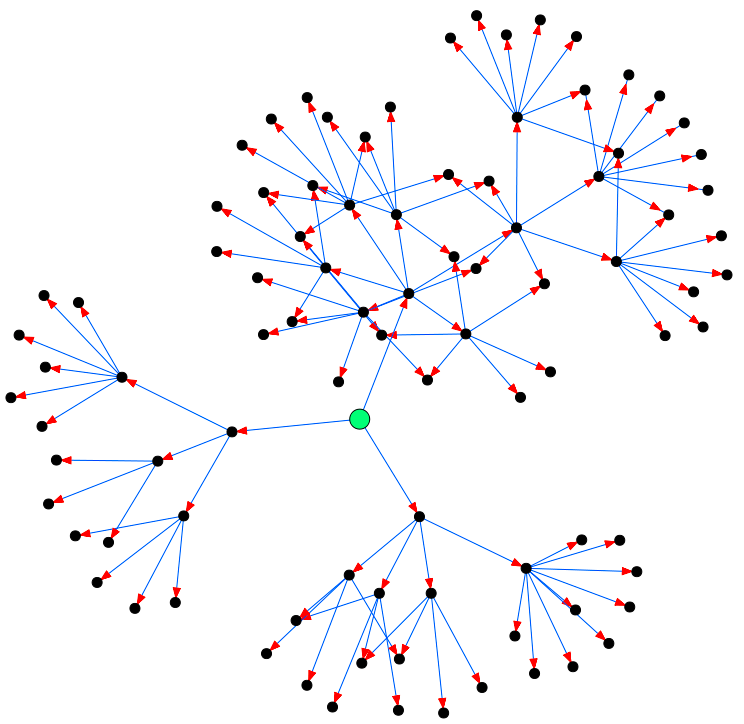
\includegraphics[height=1.2in]{Snake_4_NEATO.png}
	}
\end{figure}

}

\subsection{Cons}
\frame{\frametitle{Cons}
\begin{figure}[htbp!]
	\subfigure[(2,3)]{
		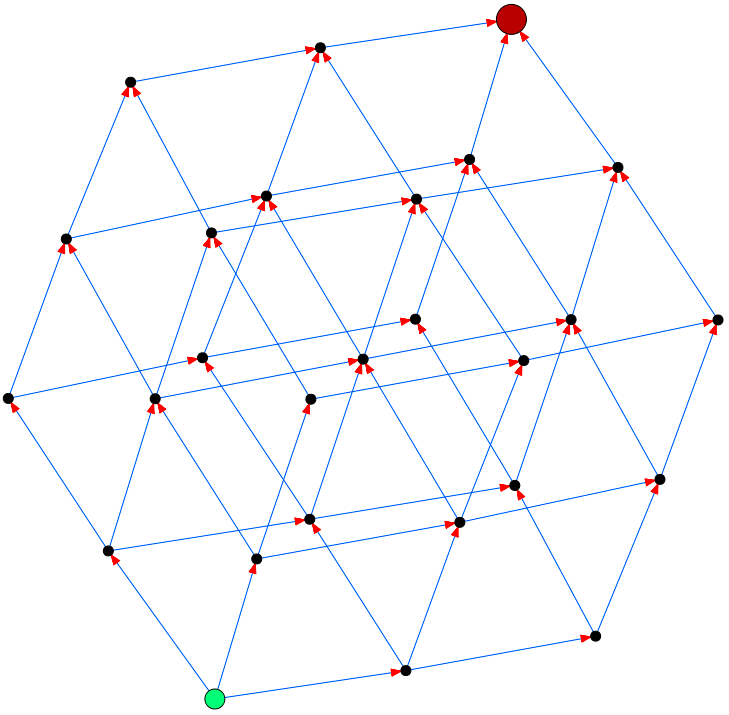
\includegraphics[height=1.2in]{Cons23_NEATO.png}
	}
	\subfigure[(4,4)]{
		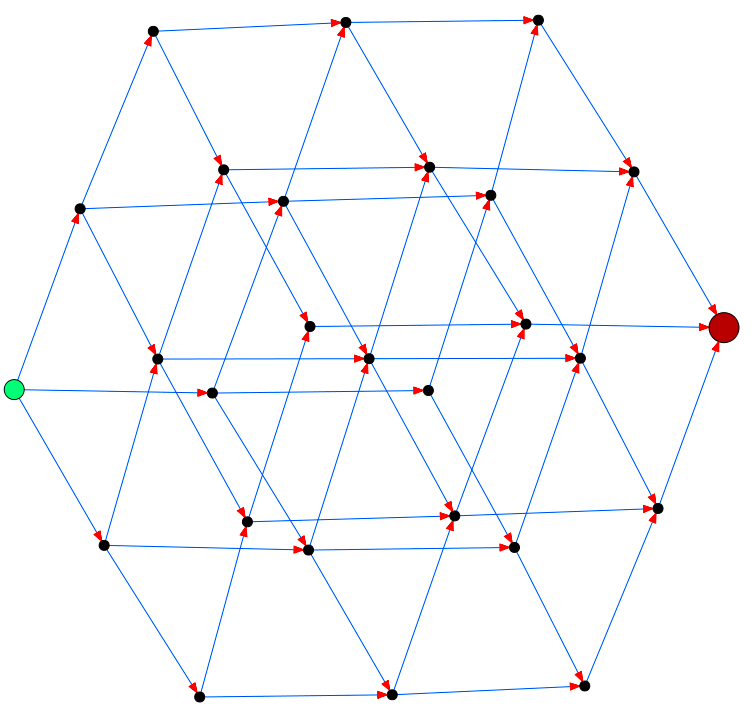
\includegraphics[height=1.2in]{Cons44_NEATO.png}
	}
	\subfigure[(5,0)]{
		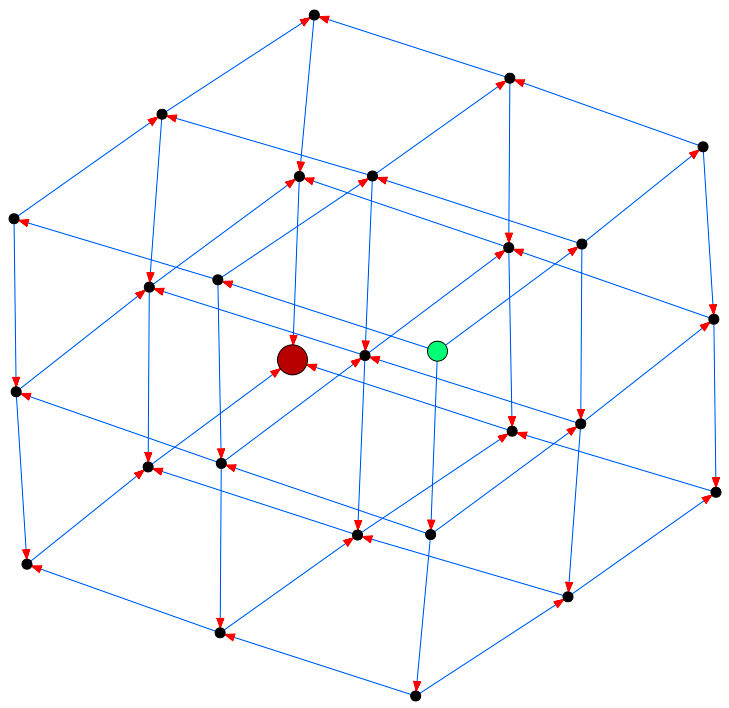
\includegraphics[height=1.2in]{Cons50_NEATO.png}
	}
	\caption{Cons funktionen}
\end{figure}
}

\section{Performance}
\frame{\frametitle{Performance}
\begin{itemize}
	\item Neato giver bedste all-round resultater 
	\item Benchmarks
\end{itemize} 
\begin{center}
	\begin{tabular}{| c | c | c | c | c | c |}
		\hline
		\multicolumn{6}{|c|}{Lambda Term: Predecessor til 4} \\
		\multicolumn{6}{|c|}{Generationsnummer: 300} \\
		\hline Neato Animated & Circo & Dot & Neato & TwoPi & Fdp \\
		\hline 4.36 & 310.44 & 0.91 & 1.11 & 0.23 & 10.90 \\
		\hline
	\end{tabular}
\end{center}
\begin{center}
	\begin{tabular}{| c | c | c | c | c | c |}
		\hline
		\multicolumn{6}{|c|}{Lambda Term: $2^2$} \\
		\multicolumn{6}{|c|}{Generationsnummer: 35} \\
		\hline Neato Animated & Circo & Dot & Neato & TwoPi & Fdp \\
		\hline 0.05 & 0.12 & 0.04 & 0.05 & 0.04 & 0.09 \\
		\hline
	\end{tabular}
\end{center}
}

\section{Fremtidigt arbejde}
\frame{\frametitle{Fremtidigt arbejde}
\begin{itemize}
	\item Udbygge med flere graftegnealgoritmer  
	\item OpenGL omskrivning (3D, zooming, etc.)
	\item Reduktionsstrategier
	\item Multitrådet
	\item Eksportering / Importering
	\item Reel brugertest
\end{itemize} 
}

\section{Konklusion}
\frame{\frametitle{Konklusion} 
\begin{itemize}
	\item En velfungerende 1. version  
	\item Gode udbyggelsesmuligheder
\end{itemize} 
}

\end{document}

